\chapter{纹理(Texturing)}
\begin{flushleft}
我们的演示渐渐变得有趣,真实世界的对象通常比每个对象的材料有更多的细节。 纹理映射是一种允许我们将图像数据映射到三角形上的技术,从而使我们能够显着增加场景的细节和真实感。 例如,我们可以通过在每一侧绘制板条纹理来构建一个立方体并将其转换为板条箱(图\ref{fig:9-1})。
\end{flushleft}

\begin{figure}[h]
    \label{fig:9-1}
    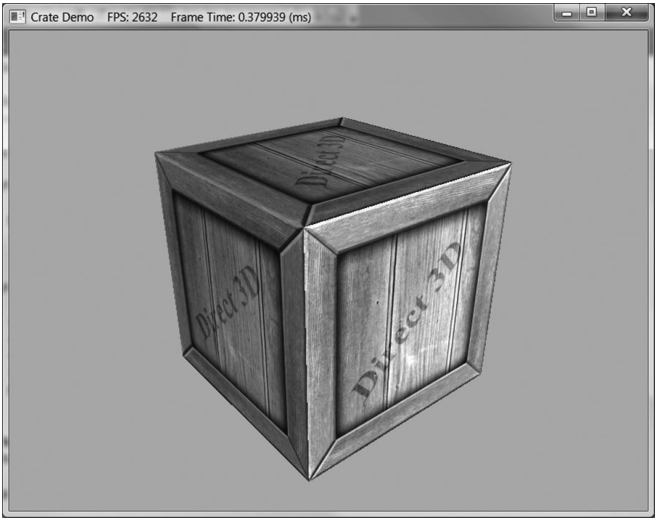
\includegraphics[width=\textwidth]{9-1}
    \centering
    \caption{Crate演示创建一个带有条板纹理的立方体。}
\end{figure}

\begin{flushleft}
当然,一般来说,模型越准确,计算成本越高; 因此,必须在现实主义和速度之间达成平衡。 例如,用于电影的3D特殊FX场景可以比游戏更复杂并且使用非常逼真的照明模型,因为电影的帧是预渲染的,因此它们可以花费数小时或数天来处理帧。 另一方面,游戏是实时应用程序,因此,帧需要以每秒至少30帧的速率绘制。\\
请注意,本书中解释和实现的照明模型很大程度上基于[Möller08]中描述的模型。\\
~\\
{\large Objectives:}
\begin{itemize}
    \item 1.了解如何指定映射到三角形的纹理部分。
    \item 2.了解如何创建并启用纹理。
    \item 3.了解如何过滤纹理以创建更平滑的图像。
    \item 4.了解如何使用地址模式多次平铺纹理。
    \item 5.了解如何组合多个纹理以创建新纹理和特殊效果。
    \item 6.学习如何通过纹理动画创建一些基本效果。
\end{itemize}
\end{flushleft}

%------- 9.1 ---------------
\section{纹理和资源回顾(Texture And Resource Recap)}
\begin{flushleft}
回想一下,自第4章以来我们已经使用了纹理; 深度缓冲区和后台缓冲区是由 ID3D12Resource 接口表示的2D纹理对象,D3D12\_RESOURCE\_DESC::Dimension 为 D3D12\_RESOURCE\_DIMENSION\_TEXTURE2D。为了便于参考,在第一部分中,我们将回顾第4章中已经介绍过的大部分纹理材料。\\

2D纹理是数据元素的矩阵。 2D纹理的一个用途是存储2D图像数据,其中纹理中的每个元素存储像素的颜色。 但是,这不是唯一的用法; 例如,在称为法线贴图的高级技术中,纹理中的每个元素都存储3D向量而不是颜色。 因此,尽管将纹理视为存储图像数据是常见的,但它们实际上更为通用。1D纹理(D3D12\_RESOURCE\_DIMENSION\_TEXTURE1D)类似于数据元素的1D阵列,3D纹理(D3D12\_RESOURCE\_DIMENSION\_TEXTURE3D)类似于数据元素的3D数组。 1D,2D和3D纹理界面均由通用ID3D12Resource表示。\\

纹理与缓冲区资源不同,缓冲区资源只存储数据数组; 纹理可以具有mipmap级别,GPU可以对它们执行特殊操作,例如应用过滤器和多重采样。 由于纹理资源支持这些特殊操作,它们仅限于某种数据格式,而缓冲资源可以存储任意数据。 纹理支持的数据格式由DXGI\_FORMAT枚举类型描述。 一些示例格式是:\\
\end{flushleft}

\begin{itemize}
  \item 1.DXGI\_FORMAT\_R32G32B32\_FLOAT:表示每个元素都是三个 32-bit的浮点型分量
  \item 2.DXGI\_FORMAT\_R16G16B16A16\_UNORM:每个元素都是四个 16-bit 的分量,取值范围在[0,1]
  \item 3.DXGI\_FORMAT\_R32G32\_UINT: 每个元素都是两个32-bit无符号整型分量
  \item 4.DXGI\_FORMAT\_R8G8B8A8\_UNORM: 每个元素都是四个 8-bit 无符号分量,取值范围在[0,1]
  \item 5.DXGI\_FORMAT\_R8G8B8A8\_SNORM: 每个元素都是四个 8-bit 有符号分量,取值范围在[-1, 1]
  \item 6.DXGI\_FORMAT\_R8G8B8A8\_SINT: 每个元素都是四个 8-bit 有符号整型分量,取值范围在[-128,127]
  \item 7.DXGI\_FORMAT\_R8G8B8A8\_UINT: 每个元素都是四个 8-bit 无符号整型分量,取值范围在[0, 255]
  \item 8.DXGI\_FORMAT\_R16G16B16A16\_TYPELESS: 每个元素都是四个 16-bit 的分量,可以在后面处理过程中,重新解释为其他类型 注:R、G、B、A分别表示red, green, blue, alpha
\end{itemize}

\begin{flushleft}
请注意,R、G、B、A字母分别代表红色、绿色、蓝色和透明度。 正如我们之前所说,纹理不需要存储颜色信息;举个例子,格式 DXGI\_FORMAT\_R32G32B32\_FLOAT 有三个浮点型分量,可以存储具有浮点坐标的3D矢量(不一定是颜色矢量)。 还有无类型格式,只保留内存,然后指定当纹理绑定到渲染管道时如何在以后重新解释数据(有点像转换); 例如,以下无类型格式保留具有四个8位分量的元素,但不指定数据类型(例如,整数,浮点,无符号整数):DXGI\_FORMAT\_R16G16B16A16\_TYPELESS。\\
~\\
NOTICE: DirectX 11 SDK文档说:“创建完全类型的资源会使资源限制为使用它创建的格式。 这使运行时能够优化访问[...]。“因此,如果您真的需要,您应该只创建无类型资源; 否则,创建一个完全类型的资源。\\
~\\
纹理可以绑定到渲染管道的不同阶段;一个常见的例子是使用纹理作为渲染目标(即Direct3D绘制到纹理中)和作为着色器资源(即,纹理将在着色器中采样)。纹理既可以用作渲染目标,也可以用作着色器资源,但不能同时使用。渲染到纹理然后将其用作着色器资源,一种称为渲染到纹理的方法允许一些有趣的特殊效果,我们将在本书后面使用它们。对于要用作渲染目标和着色器资源的纹理,我们需要为该纹理资源创建两个描述符:(1)一个存在于渲染目标堆中(即D3D12\_DESCRIPTOR\_HEAP\_TYPE\_RTV)和(2)存在于其中的一个着色器资源堆(即D3D12\_DESCRIPTOR\_HEAP\_TYPE\_CBV\_SRV\_UAV)。 (请注意,着色器资源堆还可以存储常量缓冲区视图描述符和无序访问视图描述符。)然后,资源可以绑定为渲染目标,或绑定为根签名中的根参数的着色器输入(但从不在同时):\\
\end{flushleft}

\begin{lstlisting}
// Bind as render target.
CD3DX12_CPU_DESCRIPTOR_HANDLE rtv = ...;
CD3DX12_CPU_DESCRIPTOR_HANDLE dsv = ...;
cmdList->OMSetRenderTargets(1, &rtv, true, &dsv);
// Bind as shader input to root parameter.
CD3DX12_GPU_DESCRIPTOR_HANDLE tex = ...;
cmdList->SetGraphicsRootDescriptorTable(rootParamIndex, tex);
\end{lstlisting}

\begin{flushleft}
资源描述符基本上做了两件事:它们告诉Direct3D资源将如何使用(即,您将绑定它的管道的哪个阶段),如果资源格式在创建时被指定为无类型,那么现在必须在创建视图时声明类型。 因此,对于无类型格式,纹理的元素可以在一个管道阶段中被视为浮点值,而在另一个管道阶段中被视为整数; 这基本上相当于对数据的重新解释。\\
在本章中,我们只对将纹理绑定为着色器资源感兴趣,以便我们的像素着色器可以对纹理进行采样来着色像素。\\
\end{flushleft}

%------- 9.2 ---------------
\section{纹理坐标(Texture Coordinates)}
\begin{flushleft}
Direct3D使用纹理坐标系,该坐标系包含一个水平延伸到图像的$u$轴和一个垂直于图像运行的$v$轴。 坐标$(u,v)$使得$0\leq u,v\leq 1$,将纹理上的元素称为纹素(texel)。 请注意,$v$轴在“向下”方向上为正(参见图\ref{fig:9-2})。另外,请注意使用的归一化坐标间隔$[0,1]$,因为它为Direct3D提供了与维度无关的范围; 例如,无论实际纹理尺寸是$256\times 256$,$512\times 1024$还是$2048\times 2048$像素,$(0.5,0.5)$总是指定中间纹理像素。 同样地,$(0.25,0.75)$将纹理元素识别为水平方向上总宽度的四分之一,以及垂直方向上总高度的四分之三。 目前,纹理坐标始终在$[0,1]$范围内,但稍后我们将解释当您超出此范围时会发生什么。
\end{flushleft}

\begin{figure}[h]
    \label{fig:9-2}
    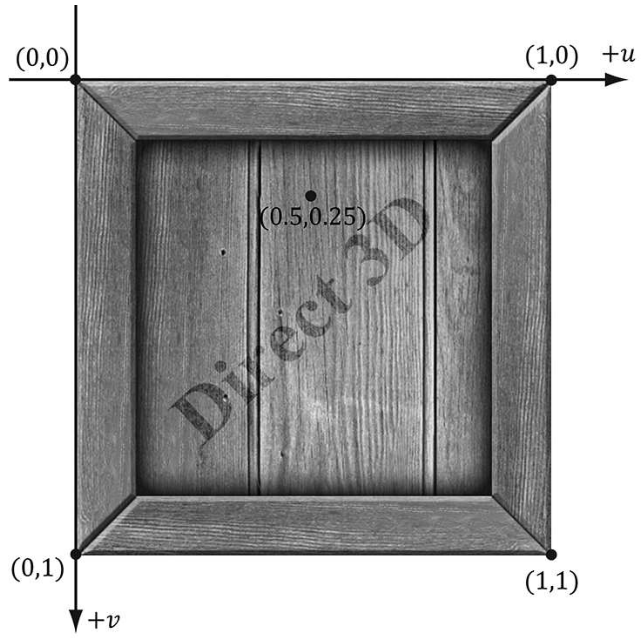
\includegraphics[width=\textwidth]{9-2}
    \centering
    \caption{纹理坐标系,有时称为纹理空间。}
\end{figure}

\begin{figure}[h]
    \label{fig:9-3}
    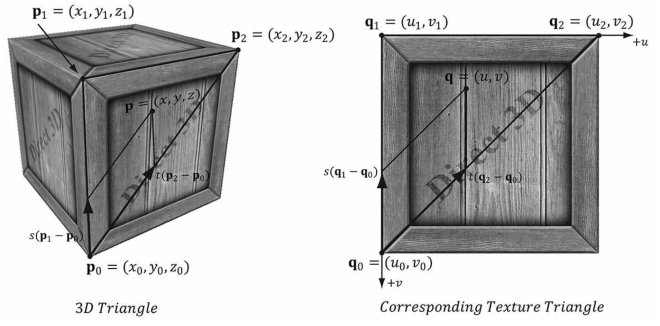
\includegraphics[width=\textwidth]{9-3}
    \centering
    \caption{左边是三维空间中的三角形,右边是我们在纹理上定义一个2D三角形,它将被映射到3D三角形上。}
\end{figure}

\begin{flushleft}
对于每个3D三角形,要在纹理上定义一个相应的三角形,以映射到3D三角形上(参见图\ref{fig:9-3})。 令$p_{0}$,$p_{1}$和$p_{2}$为具有相应纹理坐标$q_{0}$,$q_{1}$和$q_{2}$的3D三角形的顶点。 对于3D三角形上的任意点$(x,y,z)$,通过使用相同的$s$,$t$参数对3D三角形上的顶点纹理坐标进行线性插值来找到其纹理坐标$(u,v)$;即\\
如果 \\
\end{flushleft}
\begin{align*}
(x,y,z)=p=p_{0}+s(p_{1}-p_{0})+t(p_{2}-p_{0})\\
\end{align*}
\begin{flushleft}
对于 $s\geq 0,t\geq 0,s+t\leq 1$ 则,\\
\end{flushleft}
\begin{align*}
(u,v)=q=q_{0}+s(q_{1}-q_{0})+t(q_{2}-q_{0})
\end{align*}
\begin{flushleft}
这样,三角形上的每个点都有一个相应的纹理坐标。\\
为了实现这一点,需要再次修改顶点结构,并添加一对纹理坐标,用于标识纹理上的一个点。 现在每个3D顶点都有一个相应的2D纹理顶点。 因此,由三个顶点定义的每个3D三角形也在纹理空间中定义2D三角形(即,我们已经为每个3D三角形关联了2D纹理三角形)。\\
\end{flushleft}

\begin{lstlisting}
struct Vertex
{
    DirectX::XMFLOAT3 Pos;
    DirectX::XMFLOAT3 Normal;
    DirectX::XMFLOAT2 TexC;
};

std::vector<D3D12_INPUT_ELEMENT_DESC> mInputLayout =
{
    { "POSITION", 0, DXGI_FORMAT_R32G32B32_FLOAT, 0, 0,
       D3D12_INPUT_CLASSIFICATION_PER_VERTEX_DATA, 0 },
    { "NORMAL", 0, DXGI_FORMAT_R32G32B32_FLOAT, 0, 12,
       D3D12_INPUT_CLASSIFICATION_PER_VERTEX_DATA, 0 },
    { "TEXCOORD", 0, DXGI_FORMAT_R32G32_FLOAT, 0, 24,
       D3D12_INPUT_CLASSIFICATION_PER_VERTEX_DATA, 0 },
};
\end{lstlisting}

\begin{flushleft}
~\\
NOTICE: 您可以创建“奇数”纹理映射,其中2D纹理三角形与3D三角形有很大不同。 因此,当2D纹理被映射到3D三角形时,发生大量拉伸和扭曲,使得结果看起来不好。 例如,将锐角三角形映射到直角三角形需要拉伸。 通常,纹理失真应该最小化,除非纹理艺术家需要失真外观。\\
~\\
请注意,在图\ref{fig:9-3}中,我们将整个纹理图像映射到立方体的每个面上。这绝不是必需的。 可以将纹理的子集映射到几何体上。 实际上,我们可以在一个大的纹理贴图上放置几个不相关的图像(这称为纹理图集),并将其用于几个不同的对象(图\ref{fig:9-4})。 纹理坐标将决定纹理的哪个部分映射到三角形。\\
\end{flushleft}

\begin{figure}[h]
    \label{fig:9-4}
    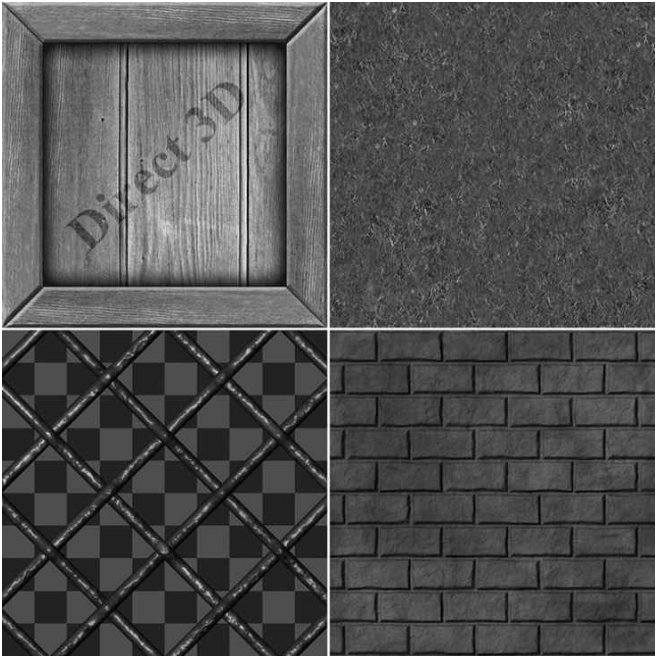
\includegraphics[width=\textwidth]{9-4}
    \centering
    \caption{在一个大纹理上存储四个子纹理的纹理图集。 设置每个顶点的纹理坐标,以便将纹理的所需部分映射到几何体上。}
\end{figure}

%------- 9.3 ---------------
\section{纹理数据源(Texture Data Sources)}
\begin{flushleft}
为游戏创建纹理的最流行的方法是让艺术家在Photoshop或其他图像编辑器中制作它们,然后将它们保存为图像文件,如BMP,DDS,TGA或PNG。 然后游戏应用程序将加载时的图像数据加载到ID3D12Resource对象中。 对于实时图形应用程序,DDS(DirectDraw表面格式)图像文件格式是首选,因为它支持GPU本身理解的各种图像格式; 特别是,它支持可由GPU本机解压缩的压缩图像格式。\\
~\\
NOTICE: 艺术家不应将DDS格式用作工作图像格式。相反,他们应该使用他们喜欢的格式来保存工作。 然后,当纹理完成时,它们会导出到DDS以用于游戏应用程序。
~\\
\end{flushleft}

%------- 9.3.1 ---------------
\subsection{DDS 概览(DDS Overview)}
\begin{flushleft}
DDS格式是3D图形的理想选择,因为它支持专门用于3D图形的特殊格式和纹理类型。 它本质上是为GPU构建的图像格式。例如,DDS纹理支持3D图形开发中使用的以下功能(尚未讨论):\\
\end{flushleft}

\begin{itemize} 
  \item 1.贴图(mipmaps)
  \item 2.GPU可以本地解压缩的压缩格式
  \item 3.纹理数组
  \item 4.立方体贴图
  \item 5.体积纹理
\end{itemize}

\begin{flushleft}
DDS格式可以支持不同的像素格式。 像素格式由DXGI\_FORMAT枚举类型的成员描述; 但是,并非所有格式都适用于DDS纹理。通常,对于未压缩的图像数据,您将使用以下格式:\\
\end{flushleft}

\begin{itemize} 
  \item 1.DXGI\_FORMAT\_B8G8R8A8\_UNORM 或 DXGI\_FORMAT\_B8G8R8X8\_UNORM:用于低动态范围的图像。
  \item 2.DXGI\_FORMAT\_R16G16B16A16\_FLOAT:用于高动态范围图像。
\end{itemize}

\begin{flushleft}
随着虚拟世界随着数百个纹理的增长,纹理的GPU内存需求迅速增加(请记住,我们需要将所有这些纹理保留在GPU内存中以便快速应用它们)。 为了帮助减轻这些内存需求,Direct3D支持压缩纹理格式:BC1,BC2,BC3,BC4,BC5,BC6和BC7:\\
\end{flushleft}

\begin{itemize} 
  \item 1.BC1(DXGI_FORMAT_BC1_UNORM):如果需要压缩支持三种颜色通道的格式,并且只需要一个1位(开/关)alpha分量,请使用此格式。
  \item 2.BC2(DXGI_FORMAT_BC2_UNORM):如果需要压缩支持三种颜色通道的格式,并且只需要一个4位alpha分量,请使用此格式。
  \item 3.BC3(DXGI_FORMAT_BC3_UNORM):如果需要压缩支持三种颜色通道的格式和8位alpha分量,请使用此格式。
  \item 4.BC4(DXGI_FORMAT_BC4_UNORM):如果需要压缩包含一个颜色通道的格式(例如,灰度图像),请使用此格式。
  \item 5.BC5(DXGI_FORMAT_BC5_UNORM):如果需要压缩支持两种颜色通道的格式,请使用此格式。
  \item 6.BC6(DXGI_FORMAT_BC6_UF16):将此格式用于压缩HDR(高动态范围)图像数据。
  \item 7.BC7(DXGI_FORMAT_BC7_UNORM):使用此格式进行高质量RGBA压缩。 这种格式显着减少了压缩法线贴图造成的错误。
\end{itemize}

\begin{flushleft}
~\\
NOTICE: 压缩纹理只能用作渲染管道的着色器阶段的输入,而不能用作渲染目标。\\
NOTICE: 因为块压缩算法适用于$4\times 4$像素块,所以纹理的尺寸必须是4的倍数。\\
~\\
同样,这些格式的优点是它们可以压缩存储在GPU内存中,然后在需要时由GPU即时解压缩。 存储压缩在DDS文件中的纹理的另一个好处是它们也占用较少的硬盘空间。
\end{flushleft}

%------- 9.3.2 ---------------
\subsection{创建 DDS 文件(Createing DDS Files)}
\begin{flushleft}
如果您不熟悉图形编程,您可能不熟悉DDS,可能更习惯使用BMP,TGA或PNG等格式。 以下是将传统图像格式转换为DDS格式的两种方法:\\
\end{flushleft}

\begin{itemize} 
  \item 1.NVIDIA为Adobe Photoshop提供了一个插件,可以将图像导出为DDS格式。 该插件可在https://developer.nvidia.com/nvidia-texture-tools-adobe-photoshop 获得。 在其他选项中,它允许您指定DDS文件的DXGI\_FORMAT,并生成贴图。
  \item 2.Microsoft提供了一个名为texconv的命令行工具,可用于将传统图像格式转换为DDS。 此外,texconv程序还有其他功能,例如调整图像大小,更改像素格式,生成mipmap及其他。 您可以在以下网站https://directxtex.codeplex.com/wikipage?title=Texconv&referringTitle=Documentation找到文档和下载链接。
\end{itemize}

\begin{flushleft}
以下示例输入BMP文件 bricks.bmp 以格式 BC3\_UNORM 输出DDS文件 bricks.dds 生成具有10个mipmap的mipmap链。
\end{flushleft}

\begin{lstlisting}
texconv -m 10 -f BC3_UNORM treeArray.dds
\end{lstlisting}

\begin{flushleft}
~\\
NOTICE:  Microsoft提供了一个名为texassemble的附加命令行工具,用于创建存储纹理数组,体积贴图和立方体贴图的DDS文件。 我们将在本书的后面部分使用此工具。其文档和下载链接可以在https://directxtex.codeplex.com/wikipage?title=Texassemble&referringTitle=Documentation 找到。\\
~\\
NOTICE: Visual Studio 2015具有内置的图像编辑器,除了其他流行的格式外,还支持DDS。 您可以将图像拖到Visual Studio 2015中,它应该在图像编辑器中打开它。 对于DDS文件,您可以查看mipmap级别,更改DDS格式以及查看各种颜色通道。\\
\end{flushleft}

%------- 9.4---------------
\section{创建并启用纹理(Creating and Enabling a Texture)}
\suhsection(加载(Loading DDS Files))



